\documentclass{article}
\usepackage{listings}

% Language setting
% Replace `english' with e.g. `spanish' to change the document language
\usepackage[english]{babel}

% Set page size and margins
% Replace `letterpaper' with`a4paper' for UK/EU standard size
\usepackage[letterpaper,top=2cm,bottom=2cm,left=3cm,right=3cm,marginparwidth=1.75cm]{geometry}

% Useful packages
\usepackage{amsmath}
\usepackage{graphicx}
\usepackage[colorlinks=true, allcolors=blue]{hyperref}

\title{Lab 3}
\author{Stephen, SJ, and Owen}

\begin{document}
\maketitle


\section{Links}

Github: \href{https://github.com/owenbean400/COS470lab3}{https://github.com/owenbean400/COS470lab3} \\
Data Set: \href{https://archive.org/download/stackexchange}{https://archive.org/download/stackexchange}

\section{Step 2}

Our first word cloud was created by taking the thirty most frequent words in the Law Stack Exchange post data. With the stop words removed, we can observe that the most prominent words in the graph are terminology most likely pertaining to the various fields of law, as seen with keywords "contract", "property", "copyright", and, of course, "law". 

\begin{center}

\includegraphics[width=3.5in]{images/image2.png}
\end{center}

One particularly interesting thing about this word cloud is that the second most common group of terms seems to be those relating to locations, as seen with "united", "states", "kingdom", "england", "wales", "germany", "european", "california", and "trademark". From this, we can infer that the users of the Law Stack Exchange are interested in subjects pertaining to law in various countries, especially with the appearance of "international", which would imply an interest beyond one's own country. 

\section{Step 3}

In our second word cloud, we have some slight differences from our first. Since this word cloud is utilizing the NLTK Porter stemmer package, we can notice some word stems in place of whole words. 

\begin{center}
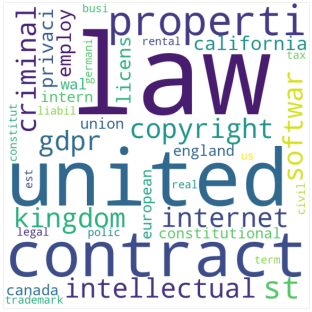
\includegraphics[width=3.5in]{images/image3.png}
\end{center}

The most interesting tokens to notice are "est", "wal", "busi", "us", and "st". For "est", "us", and "st" we can presume that these come from the ends of words, such as "best", "most", "thus" or for certain Latin words such as "corpus" and "mandamus". The word token "busi" could be derived from "business" or compound words such as "agribusiness", but may also be influenced by words such as "abusive". The token "wal" is interesting, as it is less clear what tokens other than "wales" this may have been derived from; some potential possibilities are "walk", "firewall", or "withdrawal".

\section{Step 4}

For our third graph, we are observing the frequency of the words in our dataset to determine whether our words maintain Zipf's Law, where the frequency of each word should remain proportional to its rank.

\begin{center}
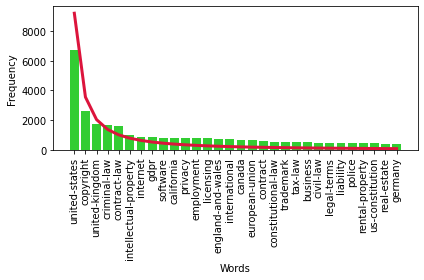
\includegraphics[width=3.5in]{images/image1.png}
\end{center}

In this dataset, we can see the frequency of each word represented by the green bars, and the red line representing the projected frequency of each word based on Zipf's Law. While we see some level of fluctuation with the words in the center of our graph, the general trend of the words seems to follow that of Zipf's Law. From this we can conclude that we have a valid collection of words for our dataset.

\end{document}